%===============================================================
% chap3.tex — Chương 3: Thiết kế kiến trúc hệ thống
%===============================================================
\pagestyle{fancy}
\chapter{THIẾT KẾ KIẾN TRÚC HỆ THỐNG}

\section{Tổng quan và kiểu hệ thống}
WebFFT là SPA không máy chủ ứng dụng: máy chủ (nếu có) chỉ phục vụ file tĩnh (\texttt{index.html}, \texttt{src/*.js}, CSS, asset). Mọi DSP và truy cập micro diễn ra trong trình duyệt người dùng. Ứng dụng có thể ``cài'' như PWA nhờ \texttt{manifest.json} và service worker \texttt{sw.js} để cache ngoại tuyến một phần tài nguyên.

\section{Phân tầng phần mềm}
\begin{itemize}\itemsep2pt
	\item \textbf{Tầng DSP thuần} (\verb|src/dsp/|): số phức, DFT, FFT/IFFT, STFT, YIN, dữ liệu butterfly --- không phụ thuộc DOM hay Web Audio, tiện kiểm thử Node.
	\item \textbf{Tầng âm thanh} (\verb|src/audioEngine.js|, \verb|src/audioWorklet/|): khởi tạo \texttt{AudioContext}, chia sẻ luồng micro, resume sau autoplay policy; worklet \texttt{pcmCapture}, \texttt{noiseReducer}.
	\item \textbf{Tầng UI theo chế độ} (\verb|src/ui/|): mỗi tab một factory (\texttt{createDftSimulatorMode}, \ldots); \verb|uiManager.js| điều phối hiển thị và vòng đời mode.
	\item \textbf{Tầng visualization} (\verb|src/visualization/|): Canvas phổ/spectrogram, SVG butterfly, vẽ tuner.
\end{itemize}

\section{Điều phối ứng dụng và điều hướng}
File \verb|src/app.js| khai báo thứ tự tab \texttt{simulator}, \texttt{analyzer}, \texttt{dtmf}, \texttt{noise}, \texttt{tuner}; đồng bộ với nút tab trong HTML và URL hash (\texttt{\#simulator}, \ldots). Khi đổi tab:
\begin{itemize}\itemsep2pt
	\item Tab không cần micro realtime (Simulator) có thể giải phóng micro và phát sự kiện \texttt{webfft:stop-audio}.
	\item Tab realtime hiển thị nhóm nút điều khiển âm thanh và ẩn/hiện theo \texttt{isRealtimeAudio}.
\end{itemize}

\section{Luồng dữ liệu âm thanh}
Hình \ref{fig:arch-webfft} minh hoạ luồng tổng quát. Micro được mở qua \texttt{getUserMedia}, đưa vào \texttt{AudioContext}. Analyzer và DTMF nhánh chính dùng \texttt{AnalyserNode} để lấy miền thời gian hoặc phổ nội bộ trình duyệt. Khử nhiễu ghép \texttt{AudioWorkletNode} với mã trong \verb|noiseReducer.js|. Simulator không bắt buộc micro; Tuner đọc PCM và gọi YIN trên main thread (buffer từ analyser hoặc capture --- xem \verb|tuner.js|).

\begin{figure}[htbp]
	\centering
	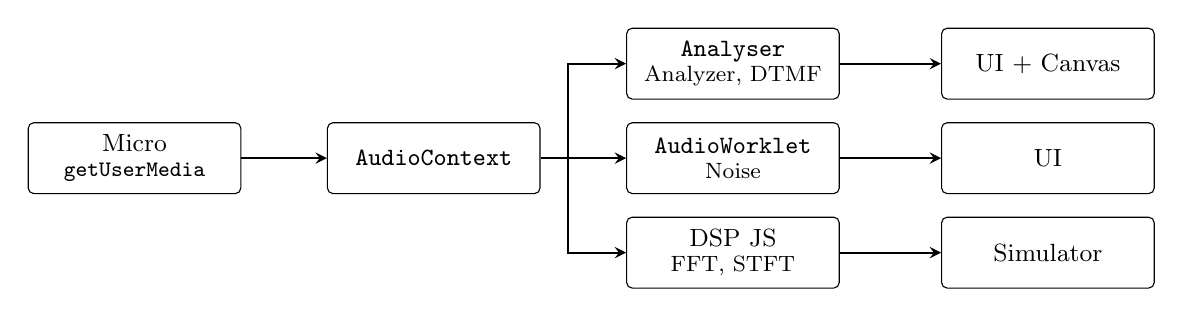
\begin{tikzpicture}[
		font=\small,
		box/.style={rectangle, draw, rounded corners=2pt, minimum width=2.7cm, minimum height=0.9cm, align=center},
		arr/.style={->, >=stealth, thick}
	]
		\node[box] (mic) at (0,0) {Micro\\[-2pt]\footnotesize\texttt{getUserMedia}};
		\node[box] (ctx) at (3.8,0) {\texttt{AudioContext}};
		\node[box] (an) at (7.6,1.2) {\texttt{Analyser}\\[-2pt]\footnotesize Analyzer, DTMF};
		\node[box] (wk) at (7.6,0) {\texttt{AudioWorklet}\\[-2pt]\footnotesize Noise};
		\node[box] (dsp) at (7.6,-1.2) {DSP JS\\[-2pt]\footnotesize FFT, STFT};
		\node[box] (ui1) at (11.6,1.2) {UI + Canvas};
		\node[box] (ui2) at (11.6,0) {UI};
		\node[box] (sim) at (11.6,-1.2) {Simulator};
		\draw[arr] (mic) -- (ctx);
		\draw[arr] (ctx.east) -- ++(0.35,0) |- (an.west);
		\draw[arr] (ctx) -- (wk.west);
		\draw[arr] (ctx.east) -- ++(0.35,0) |- (dsp.west);
		\draw[arr] (an) -- (ui1);
		\draw[arr] (wk) -- (ui2);
		\draw[arr] (dsp) -- (sim);
	\end{tikzpicture}
	\caption{Sơ đồ khối luồng dữ liệu WebFFT (đơn giản hoá).}
	\label{fig:arch-webfft}
\end{figure}

\section{Triển khai và ràng buộc môi trường}
Trình duyệt chỉ cho phép micro và \texttt{AudioContext} chạy trong ngữ cảnh bảo mật (\texttt{https} hoặc \texttt{localhost}). iOS/Safari thường yêu cầu cử chỉ người dùng trước khi phát/resume audio; tab nền có thể đình chỉ context tiết kiệm pin. Ứng dụng hiện xử lý \textbf{mono} để đơn giản hoá pipeline và khớp worklet.
